\chapter{Multi-Scale Cascade of Estimations}
%\chapter{Bayesian Compressive Sensing}
\label{ch:msce}

In this chapter, we combine the Compressive Sensing framework from Chapter \ref{ch:cs} with the Bayesian framework from Chapter \ref{ch:rvm} to form the \emph{Bayesian Compressive Sensing} (BCS) framework.

Following that, we will discuss the \emph{Multi-Scale Cascade of Estimations} (MSCE) algorithm.

\section{Bayesian Compressive Sensing}
In the Bayesian Compressive Sensing (BCS) \cite{ji2008} framework, we attempt to approach the Compressive Sensing problem from the point of view of linear regression.

Recall the setup from Chapter \ref{ch:cs}.
We are intersted in recovering the signal $\bm v\in\mathbb{R}^M$ from the CS measurements $\bm\Theta\bm v = \bm y\in\mathbb{R}^N$, where $N << M$.
We also assume that $\bm v$ is compressible in the basis $\bm \Psi$.
This means that $\bm w = \bm\Psi^T\bm v$ is well approximated by the $K$-sparse vector $\bm w_K$ which is identical to $\bm w$ for the $K$ elements in $\bm w$ with the largest magnitude.

Thus, $\bm w_e = \bm w - \bm w_K$ is assumed to be very small in magnitude in we will effectively treat it as noise,
Letting $\bm\Phi=\bm\Theta\bm\Psi$, we have
\begin{equation*}
  \bm y = \bm\Theta\bm v = \bm\Theta\bm\Psi\bm w = \bm\Phi\bm w = \bm\Phi\bm w_K + \bm\Phi\bm w_e = \bm\Phi\bm w_K + \bm n_e
\end{equation*}
where $\bm n_e = \bm\Phi\bm w_e$.
Moreover, there could be an additional noise source $\bm n$ in the CS measurements $\bm y$ (e.g. due to finite precision in the measurement device) so that, overall,
\begin{equation}
\label{eqn:bcs_setup}
  \bm y = \bm\Phi\bm w_K + \bm n_e + \bm n = \bm\Phi\bm w_K + \bm \epsilon
\end{equation}
with $\bm\epsilon = \bm n_e + \bm n$.

In the BCS literature \cite{ji2008}, $\bm\epsilon$ is typically approximated as zero-mean Gaussian noise variable with an unknown variance $\sigma^2$:
\begin{equation}
\label{eqn:bcs_noise}
  \bm\epsilon\sim\mathcal{N}(0,\sigma^2\bm I_N).
\end{equation}

Although this assumption may not always be completely accurate in practice, it is often used for its desirable analytical properties.
We might try to justify it by noting that the sensing matrix $\bm\theta$ is usually constructed randomly (often using Gaussian samples) and that the noise source $\bm n$ in the CS measurements is typically represented by a zero-mean Gaussian distribution.

Note the similarity between equations (\ref{eqn:bcs_setup}) and (\ref{eqn:bcs_noise}) and the geneneral linear regression model in equations (\ref{rvm:lklhd_2}) and (\ref{rvm:error}).
The only difference is that, in equation (\ref{eqn:bcs_setup}), we have the addtional constraint that $\bm w_K$ is \emph{sparse}.

Since in the BCS framework, we wish to solve the CS problem from a Bayesian standpoint, we are interested in computing a full posterior distribution of the weights $\bm w_K$ and the noise variance $\sigma^2$.
The sparsity constraint can be entered into the model by placing a sparseness-inducing prior distribution over the weights $\bm w_K$.

There is a range of popular sparseness priors.
Here, we choose the hierarchical prior that was specified in Chapter \ref{ch:rvm}, equations (\ref{eqn:prior_w}), (\ref{eqn:prior_alpha}) and (\ref{eqn:prior_beta}).
This allows us to use the Sparse Bayesian Learning framework to invert the CS system.

More explicitly, we view the CS measurements $\bm y \in \mathbb{R}^N$ as a target vector and $\bm\Phi=\bm\Theta\bm\Psi \in\mathbb{R}^{N\times M}$ as a design matrix and use the Sequential Sparse Bayesian Learning Algorithm (Algorithm \ref{rvm:alg2}) to compute the posterior distribution of the weights $\bm w \in \mathbb{R}^M$ (\ref{rvm:posterior}).
The desired signal $\bm v\in\mathbb{R}^M$ can then by recovered by computing 
\begin{equation}
  \label{eqn:bcs_recover}
  \bm{\hat v} = \bm\Psi\bm\mu
\end{equation} 
where $\bm \mu$ is the posterior mean of $\bm w$.

[ADVANTAGES OVER DCS?, PERFORMANCE?]

\section{Image Interpolation}
%\chapter{Multi-Scale Cascade of Estimations Algorithm}
The BCS framework of the previous section was used by \cite{pilikos2014} to reconstruct images that have missing pixel values, such as in Figure \ref{fig:lenna_mask}.
\begin{figure}
  \centering
  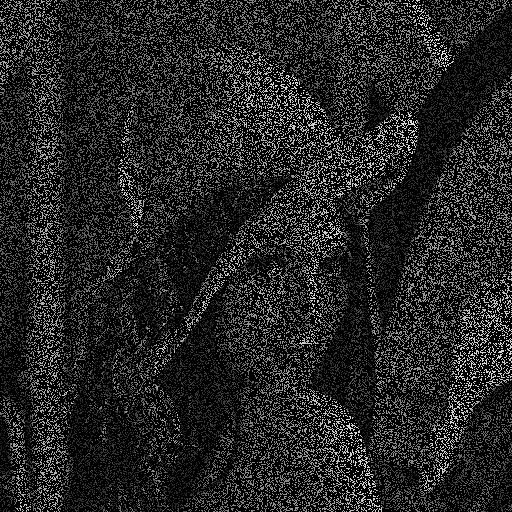
\includegraphics[width=0.6\textwidth]{Chapter5/Images/lenna_MASKED.png}
  \caption[Example of masked image signal]{Example of an image with missing pixel values. The missing data points are set to zero and displayed in black}
  \label{fig:lenna_mask}
\end{figure}

In the context of Compressive Sensing, this problem corresponds to a sensing mechanism that directly measures a down-sampled version of the original signal $\bm v$.
In Section \ref{sect:sensors} we explained how to construct corresponding sensing matrix $\bm\Theta$.
We will refer to such sensing matrices as ``masks''.
The problem of reconstructing such masked signals is sometimes also referred to as ``interpolation''.

In the BCS framework, we recover the original signal according to (\ref{eqn:bcs_recover}).
If $\bm\theta$ is a mask, the design matrix $\bm\Phi$ that is passed to the RVM consists of the basis matrix $\bm\Psi$ but with the rows corresponding to missing pixel values removed.
The recovery strategy that we discussed is thus equivalent to using the RVM directly to predict the pixel values at \emph{all} the locations according to equation (\ref{rvm:pred_mean}).

Since we have knowledge of the true pixel values for a subset of these locations, we can improve the reconstruction by replacing the predicted values with the original data when possible.

\subsection{Reconstruction using Haar Wavelets}
Using the BCS model from above with a Haar basis matrix, we reconstruct the image in Figure \ref{fig:lenna_mask}.
We display the output in Figure \ref{fig:lenna_rvm} for various scales of the Haar basis.
\begin{figure}
\centering
  \begin{subfigure}{0.4\textwidth}
    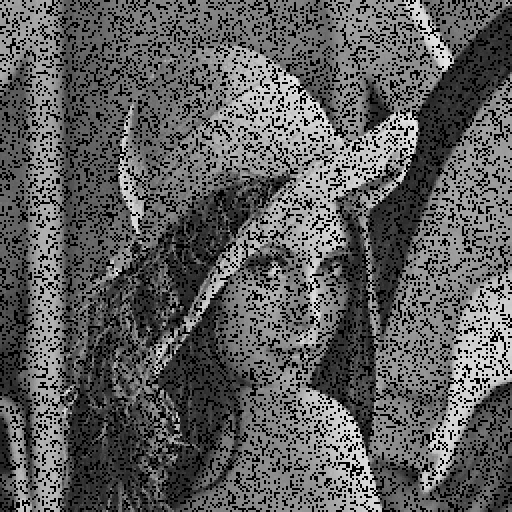
\includegraphics[width=\textwidth]{Chapter5/Images/lenna_haar1.png}
    \caption{Scale 1: PSNR = 11.75}
  \end{subfigure}
  \begin{subfigure}{0.4\textwidth}
    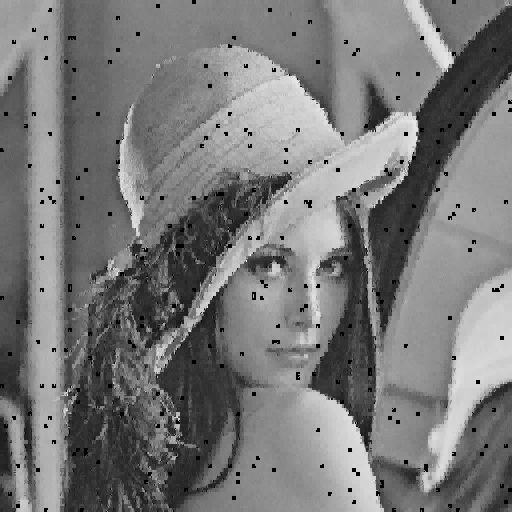
\includegraphics[width=\textwidth]{Chapter5/Images/lenna_haar2.png}
    \caption{Scale 2: PSNR = 21.78}
  \end{subfigure}
  \begin{subfigure}{0.4\textwidth}
    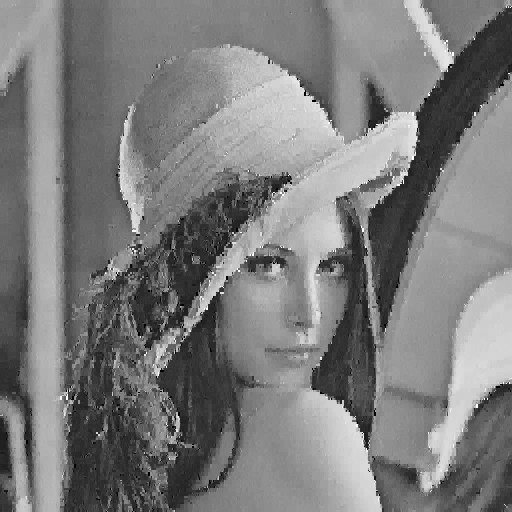
\includegraphics[width=\textwidth]{Chapter5/Images/lenna_haar3.png}
    \caption{Scale 3: PSNR = 24.15}
  \end{subfigure}
  \begin{subfigure}{0.4\textwidth}
    
\includegraphics[width=\textwidth]{Chapter5/Images/lenna_haar4.png}
    \caption{Scale 4: PSNR = 23.72}
  \end{subfigure}  
  \caption{Reconstruction if the image in Figure \ref{fig:lenna_mask} using the RVM with Haar wavelets at various scales.
    We use the \emph{Peak Signal-to-Noise Ratio (PSNR)} as our performance metric. The larger the PSNR, the more accurate the reconstruction. See Chapter \ref{ch:results} for a definition of the PSNR.}
  \label{fig:lenna_rvm}
\end{figure}

We see that the scale of the wavelet basis has a strong effect on the quality of the reconstruction.
Wavelets at lower scales can fail to reconstruct the entire image, but generally give a more accurate reconstruction at the portion of the image where they succeed.
On the other, wavelets at larger scales typically achieve a reconstruction of the entire image at the cost of increased blurring or pixelation.
This conflict can be seen in Figure \ref{fig:lenna_rvm} by contrasting panel (c) with panel (d): They both get a reconstruction of the entire image, but scale 3 actually outperforms scale 4 in this example.
Moreover, if we compare panel (b) with panel (d), we see that, in the part of the image where the recovery succeeds, the scale 2 reconstruction manages to recover finer details than both scale 3 and scale 4.

To explain why this tradeoff exists, recall that two-dimensional Haar wavelets at scale $s$ have a support of size up to $2^s\times 2^s$.
Thus, at small scales, the support of the individual basis functions is small.
For example, suppose $s=1$.
In this case, each Haar basis functions covers an area of $2\times 2$ pixels (see Figure \ref{fig:haar2_basis}).
Using these wavelets, we can capture very local relationships between the pixels.
This allows us to recover finer details in the reconstruction.

However, it can also lead to the formation of black pixels.
At scale 1, each column $j$ of the Haar basis matrix $\bm \Psi$ contains exactly 4 non-zero entries corresponding to the four pixel locations that are covered by the $j$th basis function.
If the masked image happens to be missing data at all four of these locations, the corresponding rows of the basis matrix $\bm\Psi$ will be deleted when forming the design matrix $\bm\Phi=\bm\Theta\bm\Psi$.
Therefore, column $j$ of the design matrix will be zero.
The same is true for the three columns that correspond to the remaining locations that were covered by basis function $j$.

The Sequential Sparse Bayesian Learning Algorithm will generally not select any columns that are conpletely zero, since they offer no change to marginal likelyhood.
The consequence is that the corresponding entries in the posterior mean $\bm\mu$ of $\bm w$ will remain zero.
The resulting reconstruction (\ref{eqn:bcs_recover}) will therefore be unable to recover the $2\times 2$ patch covered by basis function $j$.

This problem can be mitigated by using larger scales since, for any given number of missing pixels, it is less likely that larger square patches of the masked image are completely void of data.
However, the SSBL Algorithm generally prefers to add basis functions with larger support to the model, since they typically cause a larger increase in the Marginal Likelihood.
The result is that we get a more smoothed or blurred reconstruction and use the finer details, even in parts of the image that would have been accurately recovered at smaller scales.

\section{Multi-Scale Cascade of Estimations Algorithm}
How can we recover the finer details of the image, while also obtaining a full reconstruction?
\cite{pilikos2014} addressed this problem by using the RVM error bars to form a cascade of RVM estimations.
The resulting algorithm is called \emph{Multi-Scale Cascade of Estimations} (MSCE).

It begins by using the procedure from the previous section with the Haar basis matrix at the lowest scale to obtain a reconstruction of the masked image.
Next the error bars are computed for the predictions at the locations $\bm x^*$ of the missing pixel values:
\begin{equation}
\label{eqn:msce_error}
  (\sigma^2)^* = \sigma^2 +\bm\psi(\bm x^*)^T\bm\Sigma\bm\psi(\bm x).
\end{equation}

The MSCE algorithm uses the error measure $(\sigma^2)^*$ to decide whether to keep the estimated pixel value for location $\bm x^*$, or whether discard and keep $\bm x^*$ marked as missing.
If $(\sigma^2)^*$ is small, but larger than the noise variance $\sigma^2$, we trust the estimate and accept it. 
If $(\sigma^2)^*$ is large, we do not trust the estimate and reject it.
Finally, if $(\sigma^2)^*$ is equal to $\sigma^2$, then $\bm\psi(\bm x^*)^T\bm\Sigma\bm\psi(\bm x^*) = 0$. 
This means that $\bm\psi(\bm x^*) = 0$ since $\bm\Sigma$ is positive definite.
Thus, the RVM predicted the pixel value at location $\bm x^*$ to be zero. 
Since the recovery of the pixel was unsuccessful in this case, we reject the estimate.

If the resulting reconstruction still has missing pixel values, we pass it to the next stage of the cascade which uses a Haar basis at the next highest scale (2 in this case).

This process it repeated until we achieve a reconstruction of the entire image or until some pre-defined maximum for the scale of the Haar basis.
We have summarized the MCSE in Algorithm \ref{alg3}.

\begin{algorithm}
  \caption{Multi-Scale Cascade of Estimations \cite{pilikos2014}}
  \label{alg3}
  \begin{algorithmic}[1]
    \State Set $s=1$
    \State Let $\bm y_1 = \bm y$
    \While {$s \leq s_{max}$}
    \State Form basis matrix $\bm\Psi$ using Haar wavelets at scale $s$
    \State Call Sequential Sparse Bayesian Learning Algorithm with target
    \Statex $\qquad$ vector $\bm y_j$ and design matrix $\bm\Phi=\bm\Theta\bm\Psi$ to get the estimate $\bm{\hat v}_s$
    \State Compute $(\sigma^2)^*$ for all newly reconstructed pixel values using equation (\ref{eqn:msce_error})
    \State If $(\sigma^2)^* = \sigma^2$ or $(\sigma^2)^* > \tau$, discard the corresponding estimate
    \State Set $s = s+1$
    \State Let $\bm y_s$ be $\bm{\hat v}_s$ after the discarded estimates are deleted
    \EndWhile
    \State\Return $\bm v = \bm y_s$
  \end{algorithmic}
\end{algorithm}

